\documentclass[12pt,pdftex,16x10]{elpres} %for wide-screen slides
%\documentclass[11pt,pdftex,4x3]{elpres} %for standard 4:3 slides

\usepackage[slides]{resources/research18}
\usepackage{subcaption}

%%%%%%%%%%%%%%%%%%%%%%%%%%%%%%%%%%%%%%%%%%%%%%%%%%%%%%%%%%%% 
%%%% Footer
%%%%%%%%%%%%%%%%%%%%%%%%%%%%%%%%%%%%%%%%%%%%%%%%%%%%%%%%%%%% 
\lfoot{\parbox[l][2mm][b]{3cm}{
\includegraphics[height=4mm]{resources/isilogo_plain}}}
\cfoot{\tiny Gaspard Ulysse Fragnière}
\rfoot{\tiny\thepage}

\begin{document}

%%%%%%%%%%%%%%%%%%%%%%%%%%%%%%%%%%%%%%%%%%%%%%%%%%%%%%%%%%%% 
%%%% Title-Slide
%%%%%%%%%%%%%%%%%%%%%%%%%%%%%%%%%%%%%%%%%%%%%%%%%%%%%%%%%%%% 
\begin{titlepage}
  \centering
  \parbox{0.6\textwidth}{
\includegraphics[height=2.2cm]{resources/ethlogo_short}}
  \hfill
  \parbox{0.35\textwidth}{ 
    \mbox{}\hfill 
\includegraphics[height=1.4cm]{resources/isilogo_plain}}
  
  Master Thesis Presentation\\
  %Semester Project Presentation\\
  21 February 2023
  
  \distance{2}
  \LARGE
  \textbf{Generative Adversarial Networks for the\\
  Generation of Microphone Array Data}
  

  \normalsize
  \distance{3}
  Gaspard Ulysse Fragnière

  \distance{4}
\end{titlepage}

%%%%%%%%%%%%%%%%%%%%%%%%%%%%%%%%%%%%%%%%%%%%%%%%%%%%%%%%%%%% 
%%%%% Slides
%%%%%%%%%%%%%%%%%%%%%%%%%%%%%%%%%%%%%%%%%%%%%%%%%%%%%%%%%%%% 
\begin{psli}[Abstract]
  This thesis investigates whether Generative Adversarial Network can be used to generate realistic Cross Spectral Matrix (CSM) through their eigendecomposition. Models to generate the eigenvalues' spectrum as well the strongest eigenvector are proposed. The GAN model used to generate those quantities is a Wasserstein GAN with penalized norm of gradient of the critic with respect to its input (WGAN-GP). The method shows that WGAN-GP are suited to generate the eigenvalues spectrum and the strongest eigenvector. Based on those models, a data augmentation scheme allowing to improve the realness of synthetic CSM is introduced. Moreover, this work shows that only a few measured source cases are needed in order to generate data with properties similar to experimental data. Based on the findings of this work, GAN  could be a promising tool to achieve better generalization of deep learning models for source characterization.
\end{psli}

\begin{psli}[Agenda]
  \begin{itemize}
    \item Introduction
    \item Some Fundamentals
    \item Methods
    \item Results and Discussion
    \item Conclusion and Future Works
  \end{itemize}
\end{psli}

\begin{psli}[Introduction: Context]
  \begin{itemize}
    \item We consider the problem of source characterization and more specifically how to solve it using DL-based approaches.
    \item Unfortunately, DL-based algorithm needs significative quantities of well-structured data to be trained with.
    \item Currently data is either real measurement, synthetic data or semi-synthetic data %here explain orally what the data is and related issue
    \item Therefore new ways to obtain realistic data swiftly are needed. 
  \end{itemize}
\end{psli}

\begin{psli}[Introduction: Aim]
  \begin{itemize}
    \item First, it is relevant to note that the data used for source characterization in states of the art papers is the Cross Spectral Matrix (CSM) (e.g. in \cite{castellini2021neural}, \cite{lee2021deep}, \cite{ma2019phased}, \cite{xu2021deep}).
    \item The CSM is a direct representation of the signals received in the array of microphone.
    \item It means that recording, simulating or generating raw microphone data is not necessary, if realistic CSM could be generated directly. 
    \item Hence the goal of this thesis is to investigate the generation of the CSM directly or indirectly, as realistically as possible, using a GAN approach.
  \end{itemize}
\end{psli}

\begin{psli}[Fundamentals: Sound Model]
  \begin{minipage}[b][0.7\textheight][t]{0.5\textwidth}
    \centering
    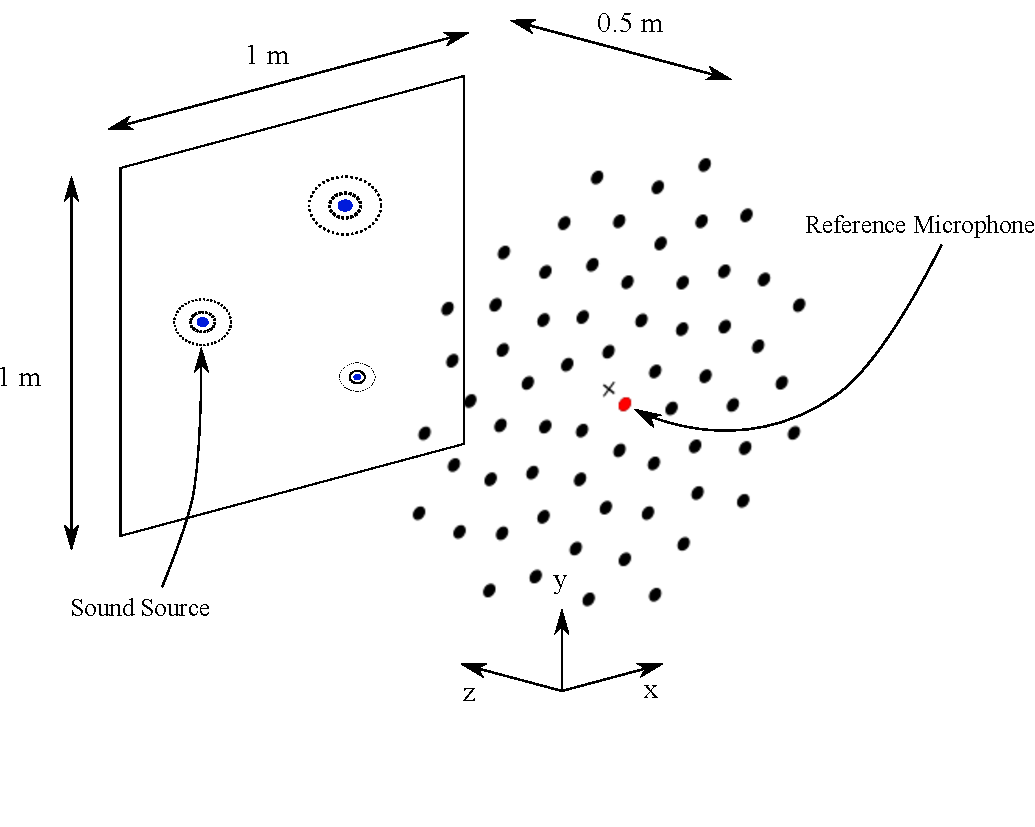
\includegraphics[width=1.1\textwidth]{figs/full_measurement_setup.pdf}
  \end{minipage}
  \begin{minipage}[b][0.7\textheight][t]{0.5\textwidth}
    \begin{itemize}
      \item  The sound model equation is given by:
    \begin{equation}
        \mathbf{p} = \mathbf{H} \mathbf{q} + \mathbf{n}
    \end{equation}
    where $\mathbf{p} \in \mathbb{C}^{64}$ is the pressure in the 64 microphones of the array, $\mathbf{q}$ the $J$ uncorrelated sources and $\mathbf{H} \in \mathbb{C}^{(64,J)}$ is the transfer function from the sources to the sensor. In this thesis, the case of a single source is considered. $\mathbf{n}$ models independent noise.
    \end{itemize}
  \end{minipage}
  
\end{psli}



\begin{psli}[Fundamentals: CSM, Eigendecomposition and Rank I CSM]
  \begin{itemize}
    \item The Cross Spectral Matrix (CSM) is a representation of the sound pressure in the different microphones. Using Welch's method, it can be approximated as:

    % Mention that the CSM is used in most beamforming algorithm.
    %Welch's method applies FFT blockwise on the array time data, calculates the CSM for each time data block and finally averages the results.
    
    \begin{equation}
        \label{csm}
        \hat{\mathbf{C}} = \frac{1}{B} \sum_{b = 1}^{B} \mathbf{p}\mathbf{p}^H
    \end{equation}
    \item A Cross spectral matrix $\hat{\mathbf{C}}$ of dimension $M \times M$ can be representated by its eigenvalues and eigenvectors using:

    \begin{equation}
        \label{eigendecomposition}
        \hat{\mathbf{C}} = \mathbf{V} \mathbf{\Lambda} \mathbf{V}^H
    \end{equation}

    \item Using only one eigenvector $\mathbf{v}_i \in \mathbf{V}$ and the corresponding eigenvalue $\mathbf{\Lambda}_{ii}$, the Rank I CSM can be computed as:
    
    \begin{equation}
        \label{rank_I_csm}
        \hat{\mathbf{C}}_i = \mathbf{v}_i \mathbf{\Lambda}_{ii} \mathbf{v}_{i}^{H}
    \end{equation}
  
  \end{itemize}
\end{psli}

\begin{psli}[Fundamentals:GAN and WGAN-GP]
  \begin{itemize}
    \item A Generative Adversial Network (GAN) is a network designed to generate realistic fake sample of some data it has been trained with.
    \item It consists of two networks competing against each other, namely a generator and a discriminator. The goal of the discriminator is to determine real from fake samples and the aim of the generator is to produce data realistic enough that the discriminator cannot determine that it has been generated.
    \item Both those inner-models are trained simultaneously. During training they both become gradually better at their tasks, until the generator becomes able to produce sufficiently realistic samples.
    \item The Wasserstein GAN with Gradient Penalty (WGAN-GP) is an improved version of the GAN. This version uses the  Wasserstein distance as loss function, which makes WGAN-GPs better at learning distribution of training data than GANs.  
  \end{itemize}
\end{psli}



\begin{psli}[Methods: Introduction]
  \begin{itemize}
    \item This thesis investiguates the generation of CSMs through their eigendecomposition
    \item This approach was chosen since CSMs are complex and hermitian matrices, it is complicated for a network to learn their distribution directly.
    \item Since there is a lack of available data, the idea is to train the generative models first using Synthetic Data and then fine-tune them using real measurement.
  \end{itemize}
\end{psli}

\begin{psli}[Methods: Data]
  \begin{minipage}[b][0.7\textheight][t]{0.5\textwidth}
    \centering
    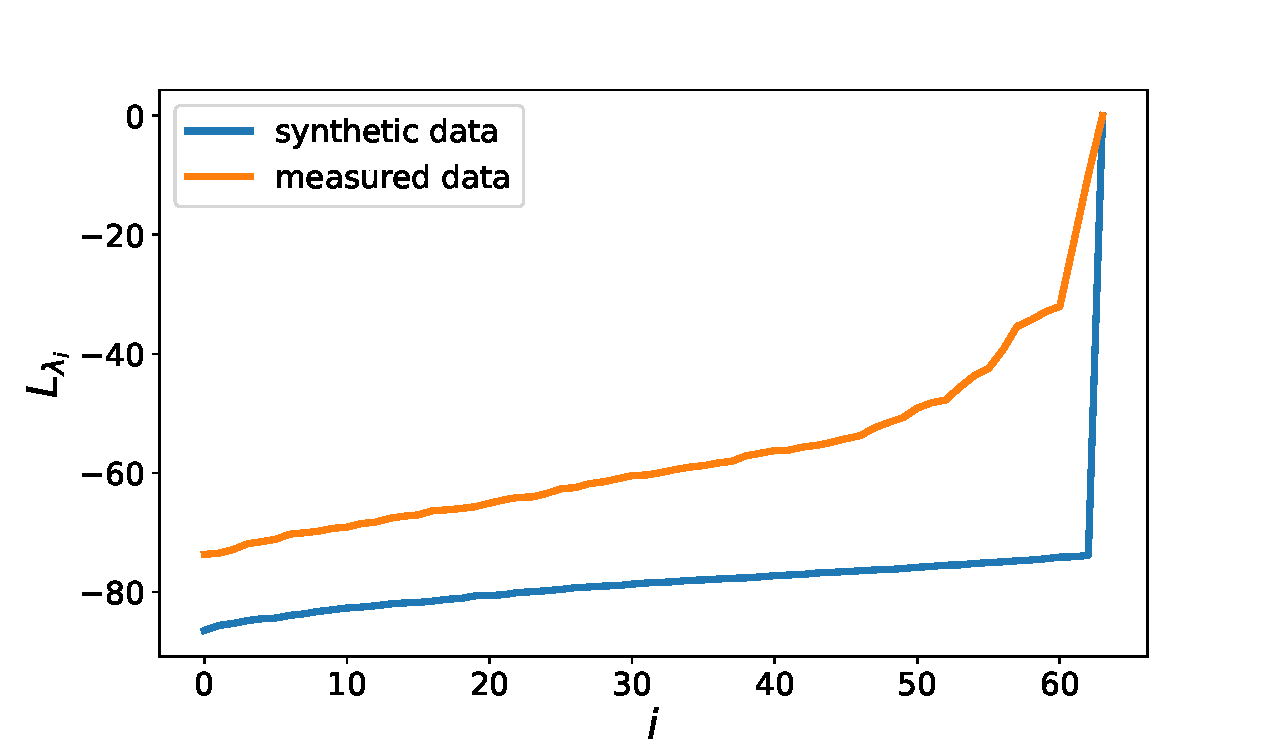
\includegraphics[width=1.2\textwidth]{figs/comparison_synthetic_measurement_data.pdf}
  \end{minipage}
  \begin{minipage}[b][0.7\textheight][t]{0.5\textwidth}
    \begin{itemize}
      \item The synthetic data has been sampled from a Wishart distribution
      \item The measurement were performed in an anechoic chamber
      \item Both the synthetic data corresponds to the same position and same Helmotz number $He = 16$
      \item The decay of the eigenvalues of synthetic data and measured data is not similar.
    \end{itemize}
  \end{minipage}
\end{psli}

\begin{psli}[Methods: Generating Eigenvalues]  
    The first approach consisted in generating the scaled eigenvalues $[\lambda_0, \dots, \lambda_{63}] \in ]0,1]^{64}$, with $\lambda_0 \leq \lambda_1 \leq \dots \leq \lambda_{63}$. This approach allowed to scale generated eigenavalues, before feeding them to the discriminator, in order to improve performances:

    \begin{figure}[htb]
      \centering
      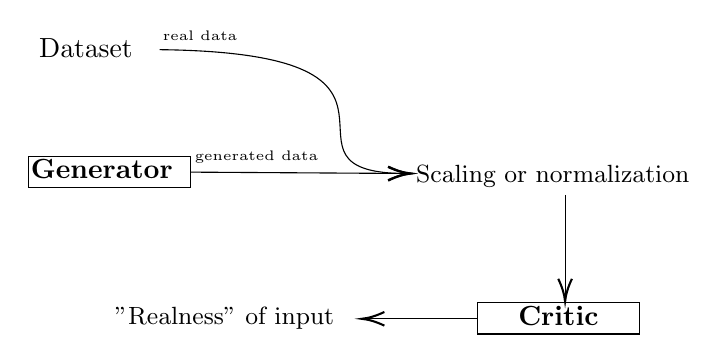
\begin{tikzpicture}[x=0.75pt,y=0.75pt,yscale=-1,xscale=1]
        %uncomment if require: \path (0,300); %set diagram left start at 0, and has height of 300
        
        %Curve Lines [id:da24102753764051987] 
        \draw    (65,9.33) .. controls (211.27,10.99) and (109.03,69.41) .. (184.84,69.01) ;
        \draw [shift={(186,69)}, rotate = 179.27] [color={rgb, 255:red, 0; green, 0; blue, 0 }  ][line width=0.75]    (10.93,-3.29) .. controls (6.95,-1.4) and (3.31,-0.3) .. (0,0) .. controls (3.31,0.3) and (6.95,1.4) .. (10.93,3.29)   ;
        %Straight Lines [id:da042737199958181704] 
        \draw    (79.67,68.33) -- (184,68.99) ;
        \draw [shift={(186,69)}, rotate = 180.36] [color={rgb, 255:red, 0; green, 0; blue, 0 }  ][line width=0.75]    (10.93,-3.29) .. controls (6.95,-1.4) and (3.31,-0.3) .. (0,0) .. controls (3.31,0.3) and (6.95,1.4) .. (10.93,3.29)   ;
        %Straight Lines [id:da48348965218999584] 
        \draw    (260.33,79.33) -- (260.33,128.67) ;
        \draw [shift={(260.33,130.67)}, rotate = 270] [color={rgb, 255:red, 0; green, 0; blue, 0 }  ][line width=0.75]    (10.93,-3.29) .. controls (6.95,-1.4) and (3.31,-0.3) .. (0,0) .. controls (3.31,0.3) and (6.95,1.4) .. (10.93,3.29)   ;
        %Straight Lines [id:da6843336271870258] 
        \draw    (218,139) -- (164.33,139) ;
        \draw [shift={(162.33,139)}, rotate = 360] [color={rgb, 255:red, 0; green, 0; blue, 0 }  ][line width=0.75]    (10.93,-3.29) .. controls (6.95,-1.4) and (3.31,-0.3) .. (0,0) .. controls (3.31,0.3) and (6.95,1.4) .. (10.93,3.29)   ;
        %Shape: Rectangle [id:dp5961208628096415] 
        \draw   (1.67,60.67) -- (79.67,60.67) -- (79.67,75.67) -- (1.67,75.67) -- cycle ;
        %Shape: Rectangle [id:dp7837205891485919] 
        \draw   (218.33,131.33) -- (296.33,131.33) -- (296.33,146.33) -- (218.33,146.33) -- cycle ;
        
        % Text Node
        \draw (1.67,61) node [anchor=north west][inner sep=0.75pt]   [align=left] {\textbf{Generator}};
        % Text Node
        \draw (236.5,131.75) node [anchor=north west][inner sep=0.75pt]   [align=left] {\textbf{Critic}};
        % Text Node
        \draw (5.67,2.67) node [anchor=north west][inner sep=0.75pt]   [align=left] {Dataset};
        % Text Node
        \draw (187.33,63.67) node [anchor=north west][inner sep=0.75pt]   [align=left] {{\small Scaling or normalization}};
        % Text Node
        \draw (80.67,56.67) node [anchor=north west][inner sep=0.75pt]   [align=left] {{\tiny generated data}};
        % Text Node
        \draw (65.33,-1) node [anchor=north west][inner sep=0.75pt]   [align=left] {{\tiny real data}};
        % Text Node
        \draw (42.33,132) node [anchor=north west][inner sep=0.75pt]   [align=left] {{\small "Realness" of input}};    
      \end{tikzpicture}
      %\caption{Full structure of the implementation used in the WGAN-GP to generate eigenvalues.}
    \label{fig:flowchart_wgangp}
  \end{figure}
\end{psli}

\begin{psli}[Methods: Generating Eigenvalues]
  \begin{itemize}
    \item The second approach to generate the eigenvalues consisted in generating their level representation $L_{\lambda_0}, \dots, L_{\lambda_{63}}$ defined as:
    \begin{equation}
        L_{\lambda_i} = 10 \log_{10}(\frac{\lambda_i}{\lambda_{63}})
    \end{equation}
    \item Since all values $L_{\lambda_i}$ are non-positive, the generator has been built such that the two last steps are first a ReLU, followed by a multiplication by $-1$. %This way it can be ensured that the network only produces non-positive spectrum. This approach was also justified by the usage of Leaky ReLU as activation throughout the generator. 
    \item Because Leaky ReLU were used in the critic, the first layer of its network is also a multiplicative layer. %Therefore, the critic is not trained to detect real from fake levels, but rather real from fake negative levels, which is equivalent.
  \end{itemize} 
  
  
\end{psli}

\begin{psli}[Methods: Generating Eigenvectors]
  \begin{itemize}
    \item In order to generate the eigenvector, it was decided to start by only generating the strongest eigenvector, as a proof of concept. We defined this eigenvector as main eigenvector.
    \item Generating only the main eigenvector can be justified by the fact, it is the most meaningful eigenvector, since it contains all the information about the position of the source. %Indeed, each eigenvector belongs to a different incoherent source. If there would to be  multiple coherent source, all the energy and their position merges into a single eigenmode. Since the case where there is only one source is under consideration, only the eigenvector with the biggest index corresponds to a DoA/source and the remaining 63 eigenvectors corresponds to noise.
    \item Since the main eigenvector is $\in \mathbb{C}^{64}$, a network with a similar architecture as the one used for the eigenvalues can be used. But instead of scaling the generated sample, they are normalized before being fed to the discriminator. %Here by normalization is meant that the main eigenvector is recomputed such that its direction remains the same but its norm is equal to 1.  
  \end{itemize}
\end{psli}

\begin{psli}[Methods: Data Augmentation]
  
  For a received synthetic CSM $\mathbf{\hat{C}}$, its  eigendecomposition $\mathbf{\hat{C}} = \mathbf{V} \mathbf{\Lambda} \mathbf{V}^H$ is computed. The CSM $\mathbf{\hat{C}}$ can then be modified with
  
  \begin{itemize}
    \item generated eigenvalues $\hat{\mathbf{\Lambda}}$, with:
    \begin{equation}
        \mathbf{\hat{C}}_\text{augm.}  = \mathbf{V} \hat{\mathbf{\Lambda}} \mathbf{V}^H
    \end{equation}

    \item a generated main eigenvector $\hat{\mathbf{v}}_M$ and corresponding semi-generated eigenvectors matrix $\hat{\mathbf{V}} = [\mathbf{v}_1^T, \dots, \hat{\mathbf{v}}_M^T]$, with:

    \begin{equation}
        \mathbf{\hat{C}}_\text{augm.}  = \hat{\mathbf{V}} \mathbf{\Lambda} \hat{\mathbf{V}}^H
    \end{equation}

  \end{itemize}

\end{psli}

\begin{psli}[Results and Discussion: Generating eigenvalues from scaled values]
  \begin{minipage}[b][0.7\textheight][t]{0.5\textwidth}
    \centering
    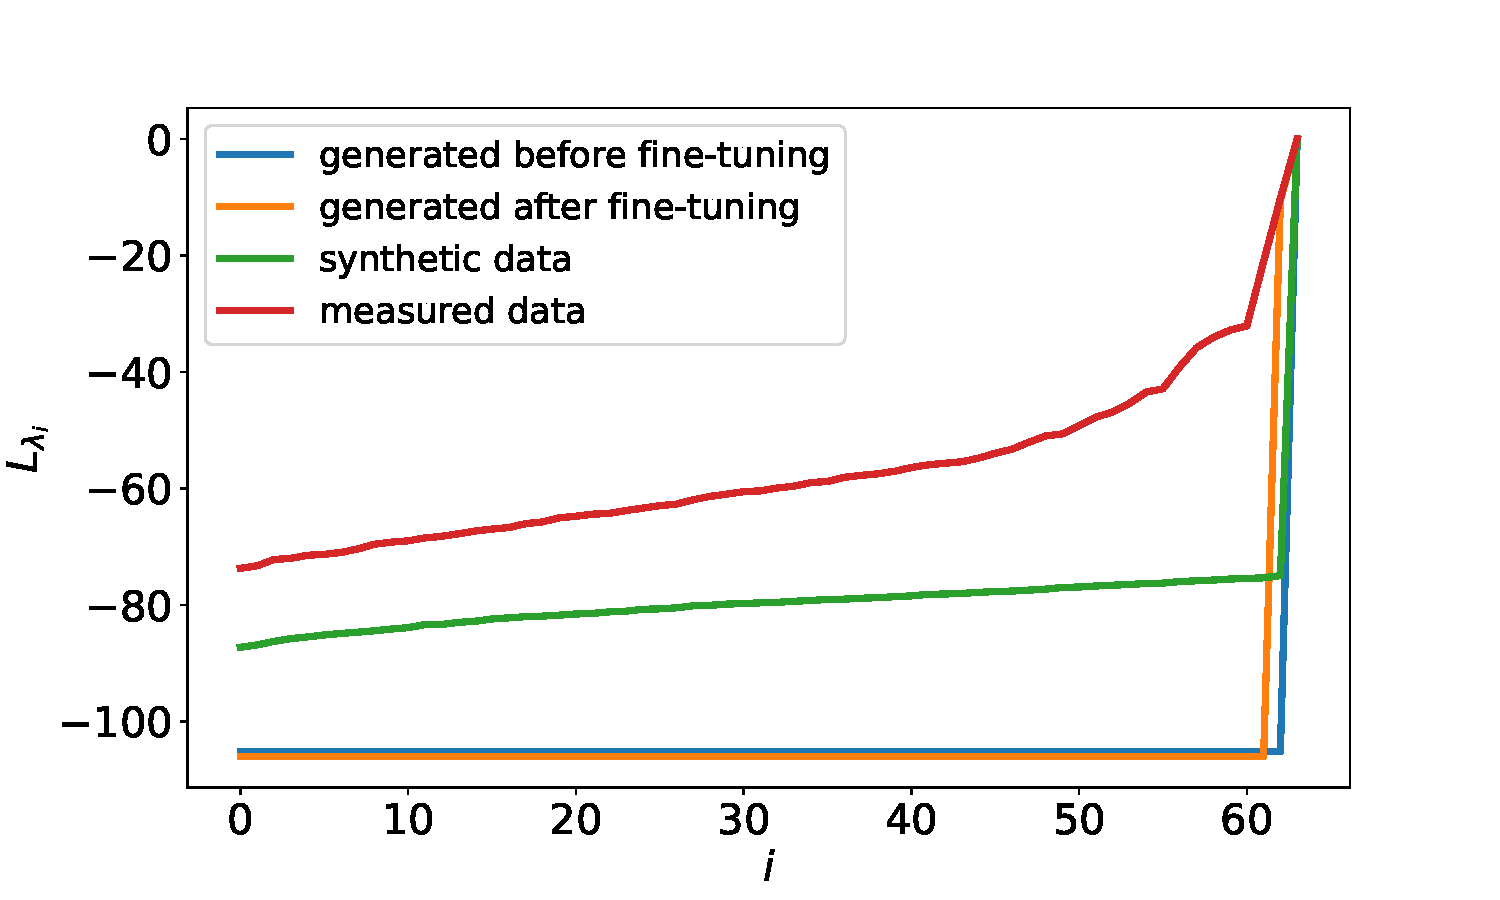
\includegraphics[width=1.2\textwidth]{figs/samples_evals_wgangp.pdf}
  \end{minipage}
  \begin{minipage}[b][0.7\textheight][t]{0.5\textwidth}
    \begin{itemize}
        \item Sudden and steep drop in value, reaching a level around $10^{-100}$
        \item Both before and after fine-tuning
        \item the WGAN-GP cannot capture very well small numerical variation
        \item This approach is not suited.
    \end{itemize}
  \end{minipage}
\end{psli}

\begin{psli}[Results and Discussion: Generating eigenvalues from levels]
  \begin{minipage}[b][0.7\textheight][t]{0.5\textwidth}
    \centering
    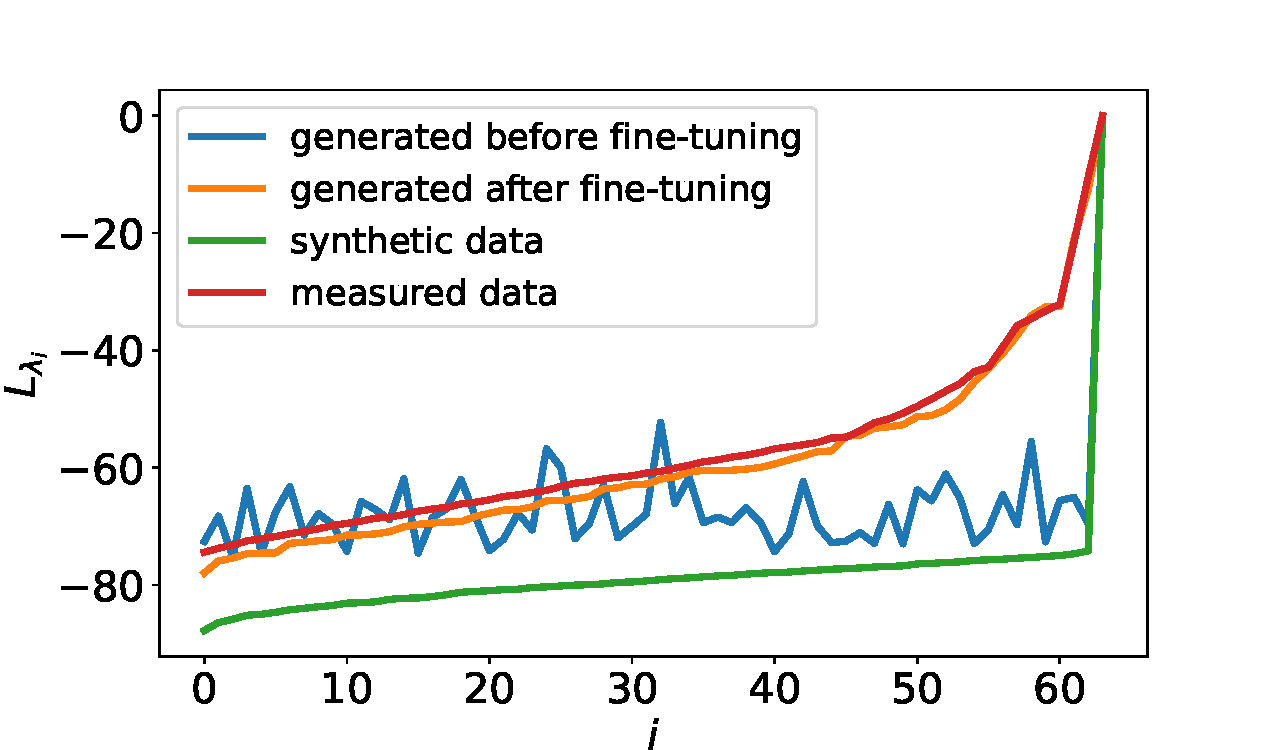
\includegraphics[width=1.2\textwidth]{figs/samples_evals_dB_wgangp.pdf}
  \end{minipage}
  \begin{minipage}[b][0.7\textheight][t]{0.5\textwidth}
    \begin{itemize}
        \item The generated data looks more like the real data, especially after fine-tuning.
        \item We conclude that generating the eigenvalues from their spectrum is the right way
    \end{itemize}
  \end{minipage}
\end{psli}

\begin{psli}[Results and Discussion: Generating eigenvalues from levels 2]
  \begin{minipage}[b][0.7\textheight][t]{0.5\textwidth}
    \centering
    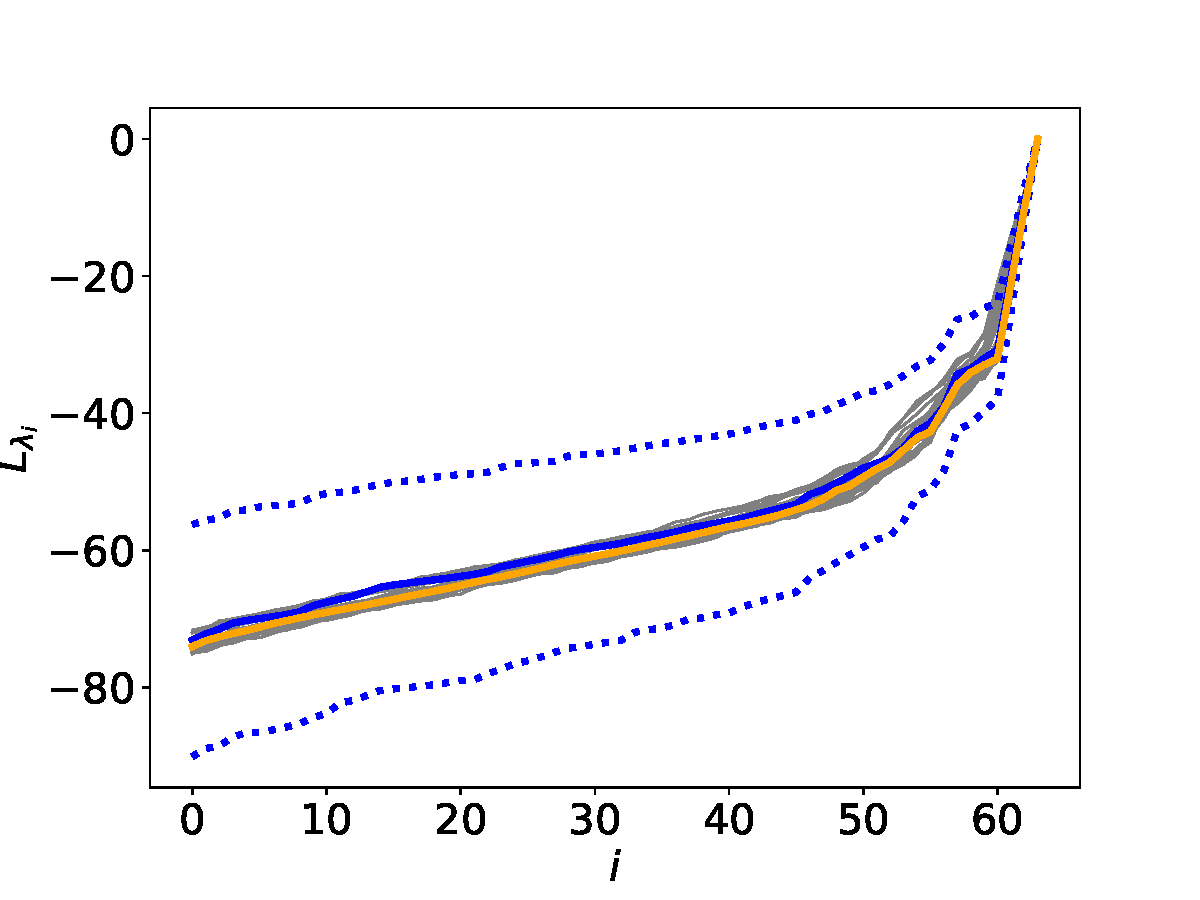
\includegraphics[width=1.2\textwidth]{figs/outliers_evals_dB_wgangp.pdf}
  \end{minipage}
  \begin{minipage}[b][0.7\textheight][t]{0.5\textwidth}
    \begin{itemize}
        \item Moreover, it was observed that training the network first with synthetic data and then fine-tuning it with a single measurement allows to produce eigenvalues with a large variation.
        \item Hence, it can be concluded that this approach allows to generate eigenvalues samples that are representative not only of a single measurement, but of multiple ones
    \end{itemize}
  \end{minipage}
\end{psli}



\begin{psli}[Results and Discussion: Generating strongest eigenvector]
  
    \begin{minipage}[t][0.3\textheight][t]{0.4\textwidth}
      \centering
      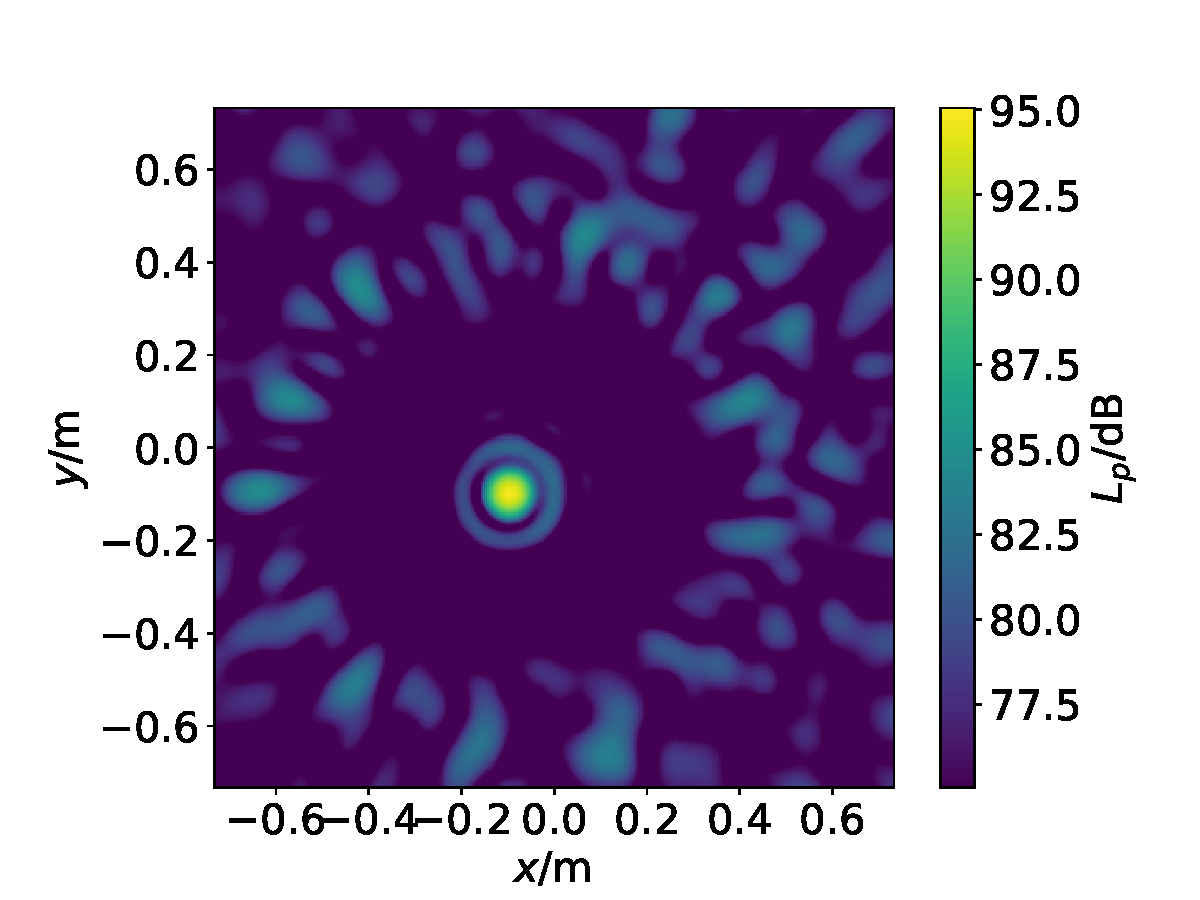
\includegraphics[width=1.2\textwidth]{figs/beamforming_map_main_evec_wgangp_generated.pdf}
    \end{minipage}
    \begin{minipage}[b][0.7\textheight][t]{0.5\textwidth}
      \begin{itemize}
          \item When observing the beamforming map computed from generated main eigenvector, it can be concluded that WGAN-GP is able to generate sufficiently realistic sample.
          \item It was observed that all the generated main eigenvector were atually pretty similar. It was therefore concluded that the WGAN-GP cannot produce a great variety of sample, but it is important to note that it is representative of the data it was trained with.  
      \end{itemize}
    \end{minipage}
  \end{psli}


% ============================================================
\begin{psli}[Results and Discussion: Data Augmentation]
  \begin{figure}
    \begin{minipage}[b]{0.4\linewidth}
      \centering
      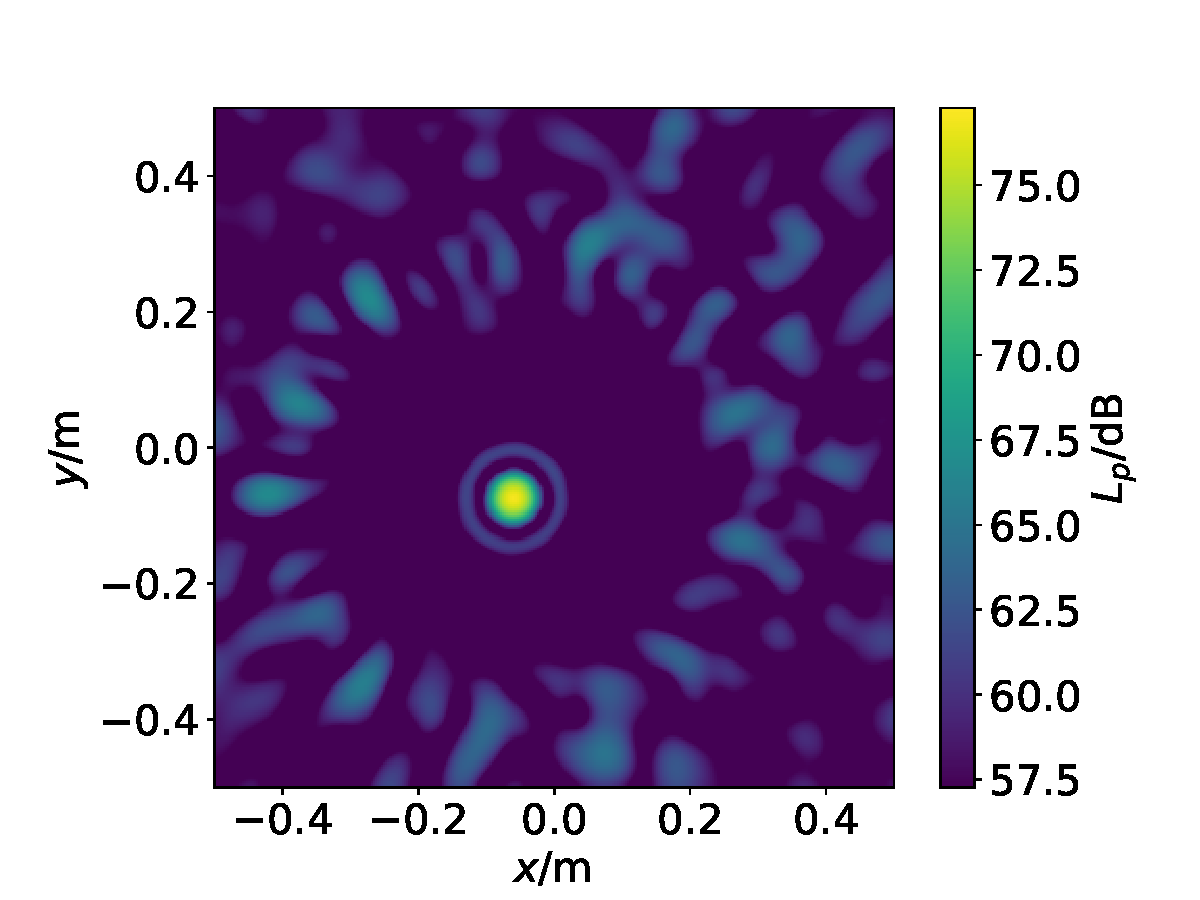
\includegraphics[width=\textwidth]{figs/datasets_beamforming_example_synthetic.pdf}
      \caption{Synthetic}
    \end{minipage}
    \begin{minipage}[b]{0.4\linewidth}
      \centering
      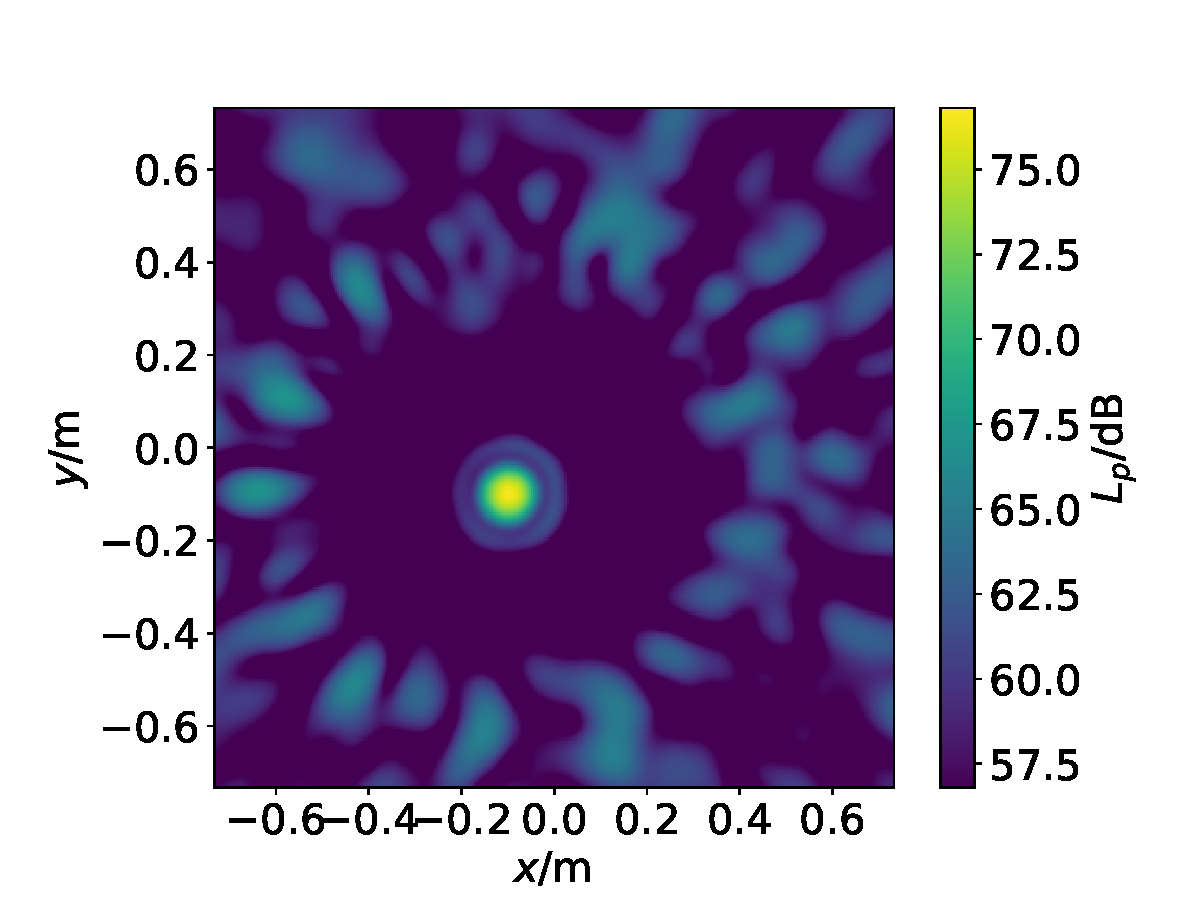
\includegraphics[width=\textwidth]{figs/datasets_beamforming_example_measurement.pdf}
      \caption{Measurement}
    \end{minipage}
    %\newline
    \begin{minipage}[b]{0.4\linewidth}
      \centering
      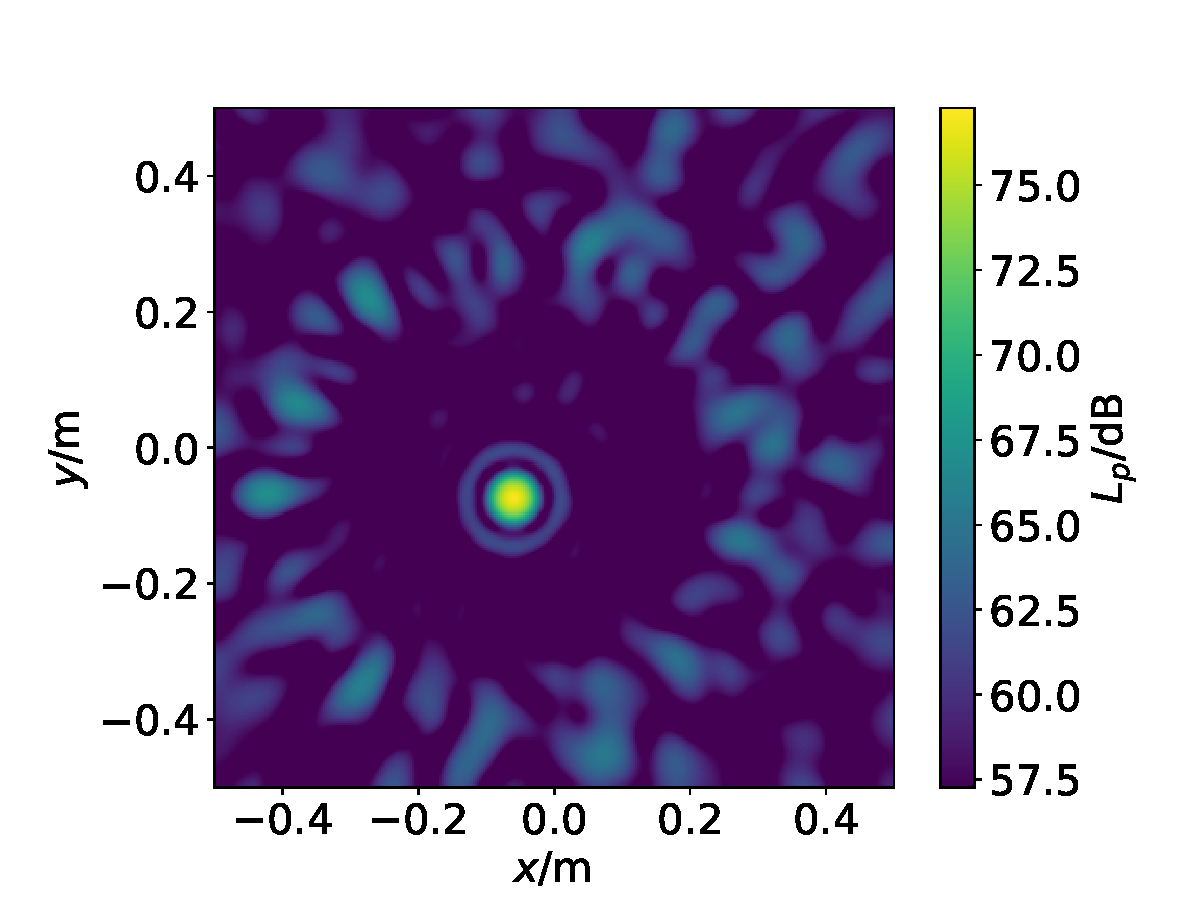
\includegraphics[width=\textwidth]{figs/data_augmentation_evals_augmented_csm.pdf}
      \caption{Augm. with eigenvalues}
    \end{minipage}
    \begin{minipage}[b]{0.4\linewidth}
      \centering
      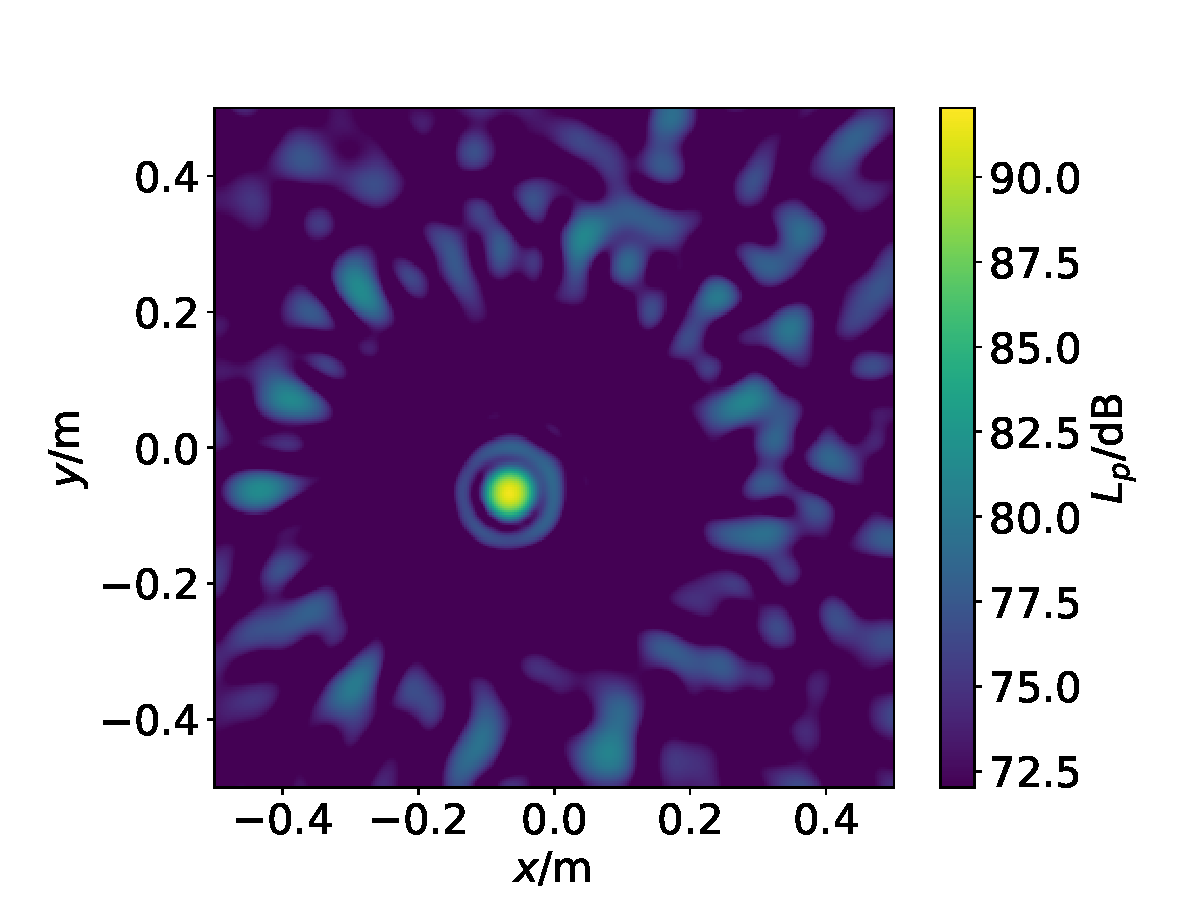
\includegraphics[width=\textwidth]{figs/data_augmentation_evecs_augmented_csm.pdf}
      \caption{Augm. with eigenvector}
    \end{minipage}
  \end{figure}
\end{psli}
% ============================================================

% ============================================================
\begin{psli}[Results and Discussion: Data Augmentation]
  \begin{figure}
    \begin{subfigure}[b]{0.5\linewidth}
      \centering
      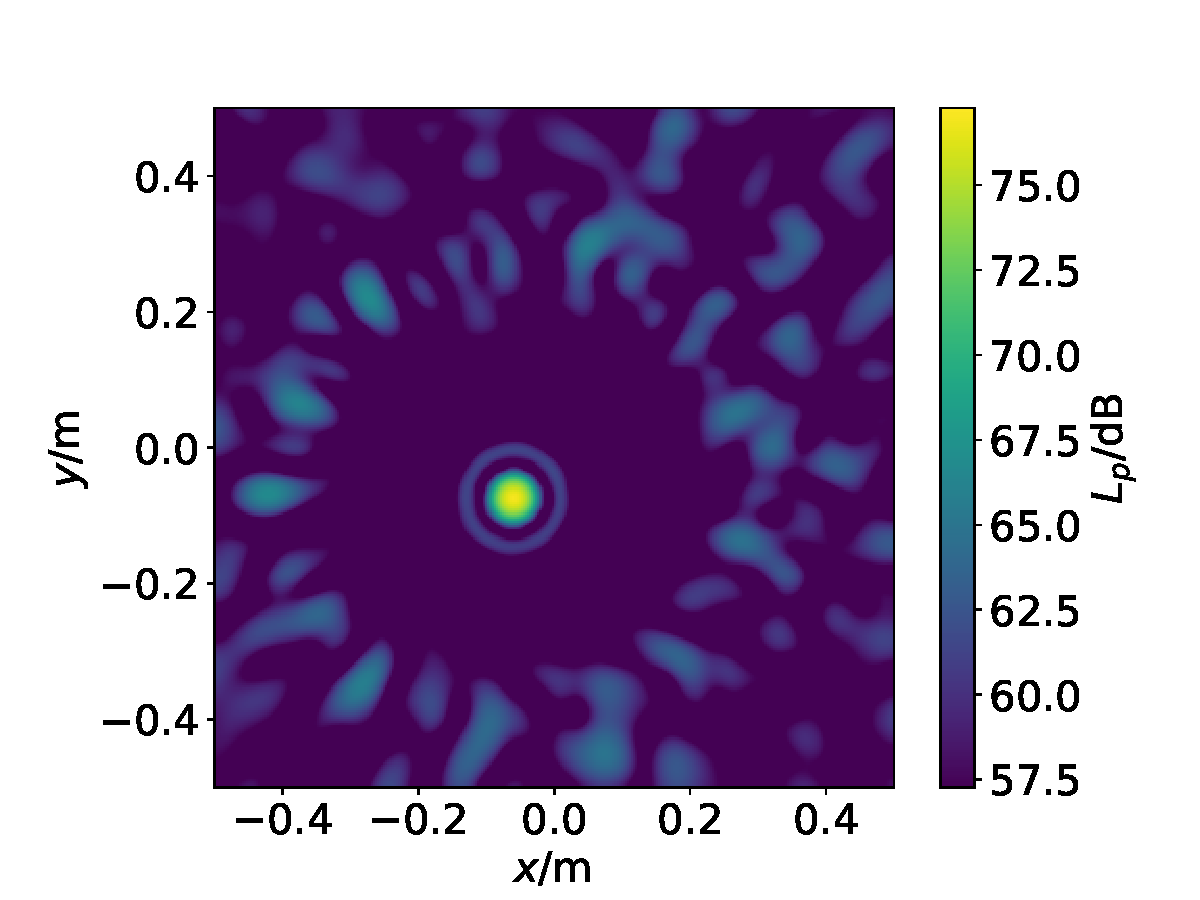
\includegraphics[width=0.75\linewidth]{figs/datasets_beamforming_example_synthetic.pdf} 
      \caption{Synthetic} 
      %\label{fig7:a} 
      %\vspace{4ex}
    \end{subfigure}%% 
    \begin{subfigure}[b]{0.5\linewidth}
      \centering
      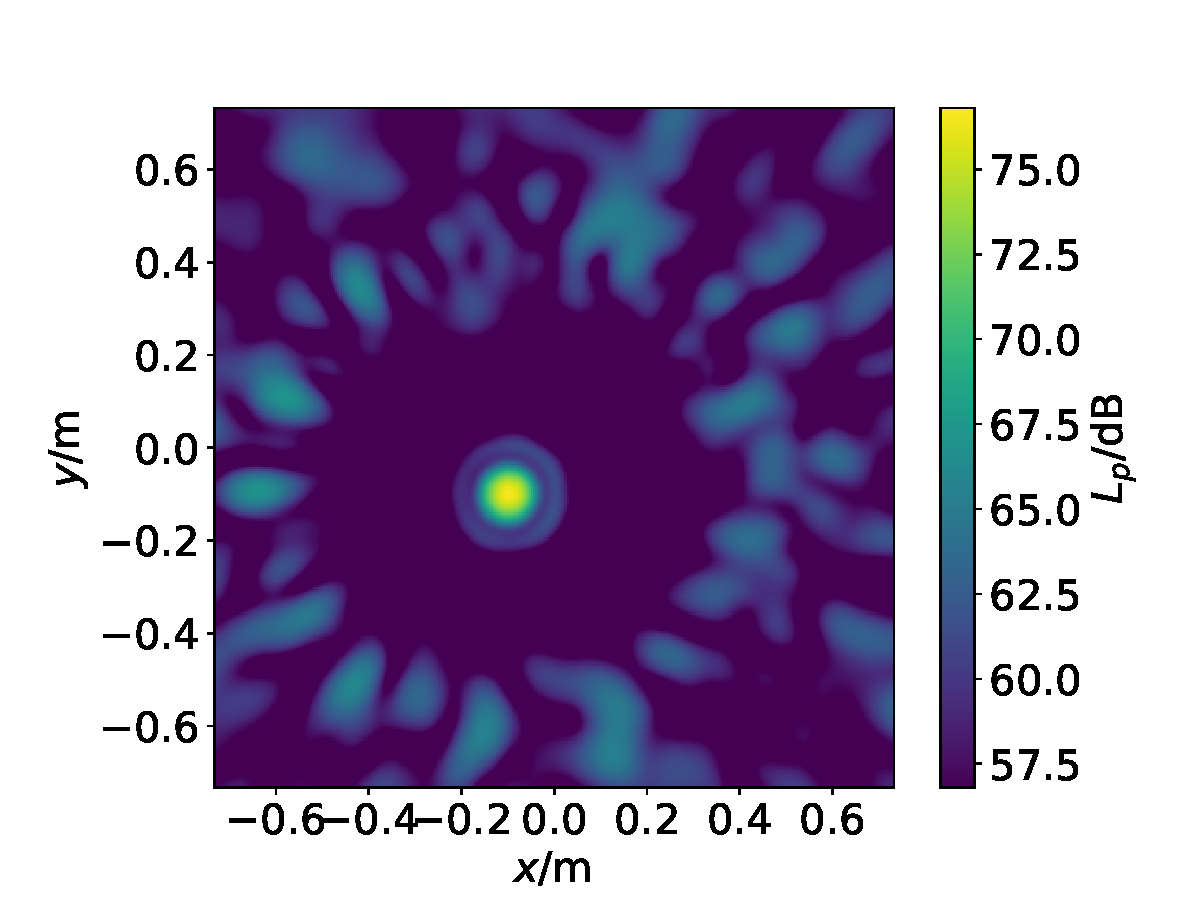
\includegraphics[width=0.75\linewidth]{figs/datasets_beamforming_example_measurement.pdf} 
      \caption{Measurement} 
      %\label{fig7:b} 
      %\vspace{4ex}
    \end{subfigure} 
    \begin{subfigure}[b]{0.5\linewidth}
      \centering
      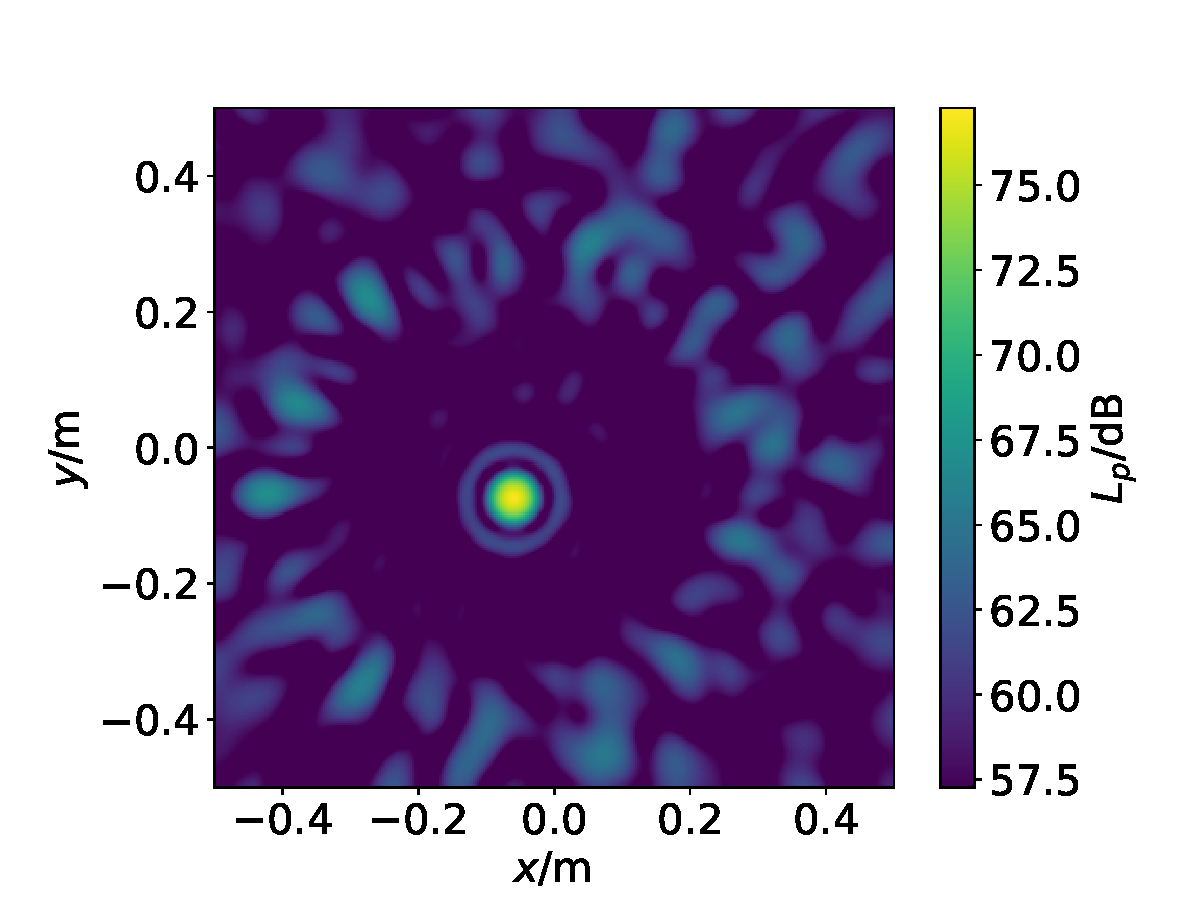
\includegraphics[width=0.75\linewidth]{figs/data_augmentation_evals_augmented_csm.pdf} 
      \caption{Augmented with Eigenvalues} 
      %\label{fig7:c} 
    \end{subfigure}%%
    \begin{subfigure}[b]{0.5\linewidth}
      \centering
      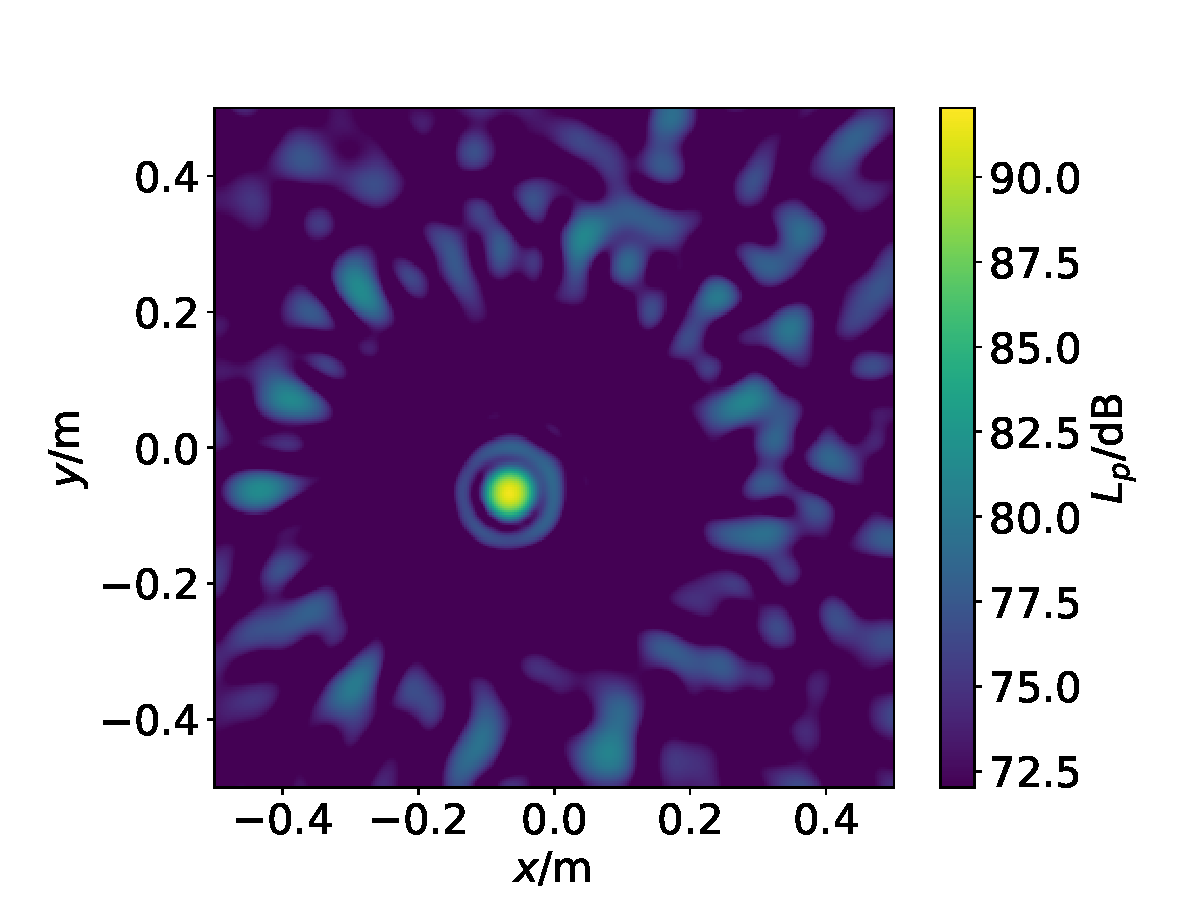
\includegraphics[width=0.75\linewidth]{figs/data_augmentation_evecs_augmented_csm.pdf} 
      \caption{Augmented with Eigenvectors}  
    \end{subfigure} 
  \end{figure}
\end{psli}
% ============================================================

\begin{psli}[Conclusion]
  \begin{itemize}
    \item It has been shown that WGAN-GPs are suited both to generate eigenvalues and strongest eigenvector. 
    \item Moreover, the data augmentation method using generated main eigenvector allows to improve how realistic synthetic CSM are.
    \item In conclusion, it can be stated that this thesis introduces new methods for learning matrix data, through eigendecomposition. It is shown that the eigedecomposition is a good representation of CSM to learn their distribution and hence generating them. 
    \item The finding in this thesis are an important step toward solving the unavailability of real training data for source localization or characterization. Indeed, as shown in the literature survey, extensive researchs on this topic do not exist, which makes the contribution of this thesis especially relevant. 
  \end{itemize}
\end{psli}

\begin{psli}[Future Works]
  \begin{itemize}
    \item Extending the work to be able to generate CSM for different positions. 
    \item More specifically, this would need to be done for the network to generate the main eigenvector. Indeed, the eigenvalue spectrum is not position dependent.
    \item More than simply training the eigenvectors for multiple positions, it should be investigated whether a Neural Network could be designed for generating eigenvectors also corresponding to a given source position not observed in the dataset.
    %It is to be noted that a good starting point for this investigation would be to attempt to build a Neural Network to learn relationship between source position and the main eigenvector.
    
    \item It also need to be investigated how to generate the remaining weakest eigenvectors. Extending the approach to generate the strongest eigenvector to all eigenvectors, has been tried but without compelling results. 
  \end{itemize}
\end{psli}

\begin{psli}
  \begin{center}
      Questions? 
  \end{center}
\end{psli}

\begin{psli}[Bibliography]
  % Bibliography
  \bibliographystyle{IEEEtran} % bibliography style in order of first citation
  \bibliography{./resources/IEEEabrv,./bibliography}
\end{psli}

\begin{psli}[Appendix]
  \begin{itemize}
    \item to fill if necessary ...
  \end{itemize}
\end{psli}



\end{document}

%%% Local Variables:
%%% mode: latex
%%% TeX-master: t
%%% End:
